\documentclass[11pt]{scrartcl}
\usepackage[sexy]{evan}
\usepackage{graphicx}
\usepackage[spanish]{babel}
\graphicspath{ {./images/} }

\usepackage{answers}
\Newassociation{hint}{hintitem}{all-hints}
\Newassociation{solu}{solutionitem}{all-solutions}
\renewcommand{\solutionextension}{out}
\renewenvironment{hintitem}[1]{\item[\bfseries #1.]}{}
\renewenvironment{solutionitem}[1]{\item[\bfseries #1.]}{}

\usepackage{venndiagram,multicol,hyperref,graphicx,array,xskak}
\usepackage{tikz}
\usetikzlibrary{positioning,trees}

\begin{document}
\title{Miscelánea}
\author{Ricardo Largaespada}
\date{09 Noviembre 2024}

\maketitle

\section{Introducción}

En las próximas dos clases, haremos un conjunto de problemas que fijarán las ideas aprendidas durante el curso. Además, no saber previamente el tema en el cual cada problema encaja sirve como entrenamiento para los diversos exámenes que existen actualmente.

\begin{example}
Dado un conjunto de 7 enteros positivos distintos cuya suma es 100, demuestre que es posible elegir tres de ellos cuya suma sea al menos 50.
\end{example}
\textit{Nota.} Este primer problema parece ser uno cuya solución se da a través del principio del palomar. Sin embargo, utilizaremos una idea un poco menos conocida, pero de importancia fundamental: el Arreglo en Orden.

\textbf{Solución.} Sean \( a < b < c < d < e < f < g \) estos números. Mostremos que \( e + f + g > 50 \). Si \( e > 15 \), entonces \( e + f + g > 16 + 17 + 18 = 51 \). Si \( e \leq 15 \), entonces \( a + b + c + d \leq 14 + 13 + 12 + 11 = 50 \); por lo tanto, \( e + f + g = 100 - a - b - c - d \geq 50 \).

\begin{example}
Dado un conjunto de \( 2n + 3 \) puntos en el plano, sin tres puntos colineales ni cuatro concíclicos, demuestre que existe un círculo que pase por tres de estos puntos de modo que existan \( n \) puntos en su interior y \( n \) puntos en su exterior.
\end{example}
\textbf{Solución.} Sean \( A \) y \( B \) dos puntos consecutivos de la envoltura convexa. Denote los demás puntos como \( P_1, P_2, \ldots, P_{2n+1} \) de tal manera que \( \angle AP_i B > \angle AP_{i+1} B \). Esto se puede hacer sin problemas, ya que no hay cuatro puntos concíclicos. Note que el círculo que pasa por los puntos \( A, B, P_{n+1} \) satisface las condiciones del problema. \qed

\begin{example}
Demuestre que existe un conjunto \( S \) de \( 3^{1000} \) puntos en el plano tal que, para cada punto \( P \) de \( S \), existen al menos 2000 puntos en \( S \) cuya distancia a \( P \) es exactamente una unidad.
\end{example}
\textbf{Solución.} Mostraremos, por inducción sobre \( k \), que existe un conjunto \( S_k \) de \( 3^k \) puntos en el plano tal que cada punto de \( S_k \) dista una unidad de al menos \( 2k \) puntos de \( S_k \). \qed

Tomando \( k = 1000 \), probamos el problema.

\textbf{Caso inicial}
Tome \( S_1 \) como los vértices de un triángulo equilátero de lado 1.

\textbf{Hipótesis de inducción}
Suponga la existencia de \( S_k \), como se describe, para algún \( k \geq 1 \).

\textbf{Paso inductivo}
Sea \( v \) un vector. A partir de cada punto \( P \) de \( S_k \), construya un triángulo equilátero \( \Delta P \) de lado 1 en la dirección de \( v \). Si \( v \) se puede elegir de modo que los vértices de \( \Delta P \) y \( \Delta Q \) no coincidan siempre que \( P \neq Q \), entonces el conjunto \( S_{k+1} \) formado por los vértices de todos los triángulos \( \Delta P \), \( P \in S_k \), satisface el problema. Para demostrar esto, note que inicialmente \( S_{k+1} \) no es más que la unión de \( S_k \) y dos traslaciones de \( S_k \) de una unidad cuyas direcciones forman un ángulo de 60°. Así, \( S_{k+1} \) tiene \( 3 \cdot 3^k = 3^{k+1} \) puntos, y cada punto de \( S_{k+1} \) dista una unidad de al menos \( 2(k + 1) \) puntos de \( S_{k+1} \): \( 2k \) debido a la propiedad de \( S_k \) y 2 debido a la construcción de los triángulos \( \Delta P \).

Para elegir \( v \), basta tomarlo en una dirección distinta a todas las direcciones de pares de puntos de \( S_k \). Esto se puede hacer porque la cantidad de direcciones de pares de puntos de \( S_k \) es finita. \qed

\begin{example}[Rioplatense 2003]
Sobre una mesa hay \( n \geq 2 \) bolsas de plástico, todas de colores distintos. Cada una está en contacto con la mesa o está dentro de otra bolsa. La operación permitida es elegir una bolsa que está en contacto con la mesa, retirar todas las bolsas de su interior y colocarlas sobre la mesa, y colocar todas las otras bolsas que estaban fuera dentro de ella (sin modificar el contenido de las otras bolsas). Determine el total de configuraciones diferentes que se pueden obtener utilizando la operación cuantas veces sea necesario.
\end{example}
\textbf{Solución.} Construya un grafo con \( n \) vértices, donde cada vértice representa una bolsa. Vamos a conectar dos vértices \( v_i, v_j \) si las bolsas \( b_i, b_j \) están inmediatamente una dentro de la otra. El grafo será similar al grafo siguiente.
\vspace{-.3cm}
\begin{center}
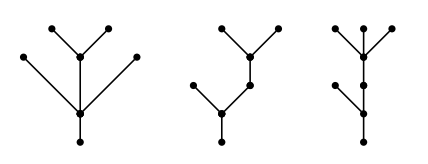
\includegraphics[scale=1]{images/clase_20_1.png}
\end{center}
\vspace{-.5cm}
Ahora construya un nuevo vértice \( F \) y conéctelo a todos los vértices que representan las bolsas que están sobre la mesa. Note que aplicar la operación en el grafo representa intercambiar la posición del vértice \( F \) por la posición del vértice que fue operado. Y como el grafo tiene un total de \( n + 1 \) vértices, existen en total \( n + 1 \) configuraciones. \qed
\vspace{-.3cm}
\begin{center}
    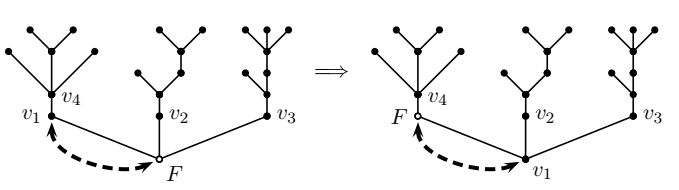
\includegraphics[scale=1]{images/clase_20_2.png}
\end{center}
\vspace{-.5cm}
La figura anterior muestra el intercambio de posiciones de los vértices \( F \) y \( v_1 \). Los vértices \( v_1, v_2, v_3 \) representan las tres bolsas que estaban inicialmente sobre la mesa. Note que, después de aplicar la operación, los vértices conectados a \( F \) son \( v_1 \) y \( v_4 \), y las bolsas que quedan sobre la mesa son exactamente \( b_1 \) y \( b_4 \).

\begin{example}[URSS 1990]
Suponga que existen 1990 pilas, consistentes en 1, 2, ..., 1990 piedras, respectivamente. En un movimiento, se puede elegir algunas pilas (posiblemente solo una) y retirar de cada pila elegida una cantidad fija de piedras. ¿Cuál es el menor número de movimientos necesarios para retirar todas las piedras de todas las pilas?
\end{example}
\textbf{Solución.} Separe las pilas en grupos con la misma cantidad de piedras, donde las pilas vacías forman su propio grupo. De esta forma, inicialmente tenemos 1990 grupos distintos. Supongamos que en un momento dado existen \( n \) grupos de pilas y realizamos un movimiento que consiste en retirar una misma cantidad de piedras de pilas que están en \( k \) grupos diferentes. Este grupo de pilas que realizamos la operación continúa representando \( k \) grupos diferentes. Además, las demás pilas de los restantes \( n - k \) grupos que no fueron alterados siguen representando \( n - k \) grupos distintos. De esta forma, tras realizar un movimiento que altera pilas de \( k \) grupos, tenemos al menos \( \max(n-k, k) \) grupos en el próximo momento. Por lo tanto, el número de diferentes grupos no decrece más rápido que la siguiente secuencia:

\[
995, 498, 249, 125, 63, 32, 16, 8, 4, 2, 1.
\]

Así, necesitamos utilizar al menos 11 movimientos.

Ahora demostraremos que es posible retirar todas las piedras usando exactamente 11 movimientos. Sea \( m_n \) el movimiento que retira \( n \) piedras de cada pila que tiene \( n \) piedras o más. Ahora considere la secuencia de movimientos:

\[
m_{995}, m_{498}, m_{249}, m_{125}, m_{63}, m_{32}, m_{16}, m_{8}, m_{4}, m_{2}, m_{1}.
\]

Es fácil verificar que esta secuencia es capaz de retirar todas las piedras. \qed

\section{Problemas Propuestos}

\Opensolutionfile{all-hints}

\section*{Problemas Propuestos}

\begin{problem}
Considere un conjunto de \(2n + 2\) puntos en el plano, no colineales. Demuestre que se pueden elegir dos de estos puntos de tal manera que la recta que los une divida el resto del conjunto en dos partes con \(n\) puntos cada una.
\begin{hint}
Piense en las líneas determinadas por pares de puntos del conjunto. Al variar estos pares, puede encontrar una recta que divida el conjunto restante de puntos en dos grupos iguales de \(n\) puntos cada uno.
\end{hint}
\end{problem}

\begin{problem}
Dado un conjunto de 69 enteros positivos distintos menores que 101, demuestre que se pueden elegir cuatro de ellos \(a, b, c, d\) tales que \(a < b < c\) y \(a + b + c = d\). ¿Es esto también cierto para 68 números?
\begin{hint}
Utilice el principio del palomar considerando las posibles sumas \(a + b + c\). Compare el número de combinaciones posibles con el rango de valores que \(d\) puede tomar, y observe que debe existir al menos una coincidencia.
\end{hint}
\end{problem}

\begin{problem}[USAMO 1996] Dado un conjunto de \(n\) enteros positivos, considere todas las sumas posibles formadas por uno o más de ellos. Demuestre que todas estas sumas se pueden dividir en \(n\) grupos de tal manera que, en cada grupo, la razón entre el mayor elemento y el menor no exceda 2.
\begin{hint}
Asigne cada suma al número más pequeño que la compone. Al agrupar las sumas de esta manera, analice cómo se relacionan las sumas dentro de cada grupo y demuestre que la razón entre el mayor y el menor no supera 2.
\end{hint}
\end{problem}

\begin{problem}
Demuestre que cualquier triángulo se puede dividir en \(n \geq 4\) triángulos isósceles.
\begin{hint}
Intente seleccionar puntos adecuados en los lados del triángulo y trace líneas hacia los vértices para formar triángulos isósceles. Ajuste la posición de estos puntos para lograr que los triángulos resultantes sean isósceles.
\end{hint}
\end{problem}

\begin{problem}
Demuestre que un cuadrado se puede dividir en \(n \geq 6\) cuadrados menores. Demuestre que esto no se puede hacer para \(n = 5\).
\begin{hint}
Explore diferentes formas de subdividir un cuadrado en cuadrados más pequeños, considerando configuraciones que utilicen cuadrados de distintos tamaños. Analice por qué es imposible lograr esta subdivisión con solo 5 cuadrados.
\end{hint}
\end{problem}

\begin{problem}[Rumania 1978] Demuestre que un cubo se puede dividir en \(n \geq 55\) cubos menores.
\begin{hint}
Considere métodos para particionar el cubo en cubos más pequeños, quizás utilizando un patrón o disposición que permita alcanzar al menos 55 cubos en total.
\end{hint}
\end{problem}

\begin{problem}
Un rectángulo \(R\) está cubierto por rectángulos menores (con lados paralelos a los del rectángulo \(R\)) cada uno de los cuales tiene al menos un lado entero. Demuestre que \(R\) también tiene un lado entero.
\begin{hint}
Sume las longitudes de los lados enteros de los rectángulos menores a lo largo de las dimensiones de \(R\). Esto le ayudará a demostrar que \(R\) debe tener al menos un lado de longitud entera.
\end{hint}
\end{problem}

\begin{problem}[San Petersburgo 2000] En un tablero infinito se colocan 111 L-triminos sin superposición de tal manera que cualquier cuadrado de \(2 \times 2\) que los cubra esté completamente cubierto por estos L-triminos. Demuestre que se pueden retirar algunos de ellos (pero no todos) de manera que la propiedad siga siendo válida.
\begin{hint}
Identifique áreas donde varios L-triminos contribuyen a cubrir las mismas regiones. Al encontrar estas redundancias, puede retirar ciertos L-triminos sin afectar la cobertura completa de los cuadrados \(2 \times 2\).
\end{hint}
\end{problem}

\begin{problem}[San Petersburgo 2000] En cada celda de un tablero de \(8 \times 8\) se escribe un número real positivo tal que la suma de los números en cada fila es 1. Se sabe que, para cualesquiera ocho celdas (no dos en la misma fila o columna), el producto de los números en estas celdas no es mayor que el producto de los números en la diagonal principal. Demuestre que la suma de los números en la diagonal principal es al menos 1.
\begin{hint}
Considere todas las permutaciones de columnas y compare los productos de los números seleccionados con el producto en la diagonal principal. Utilice desigualdades como la desigualdad de las medias aritmética y geométrica para relacionar las sumas y productos involucrados.
\end{hint}
\end{problem}

\Closesolutionfile{all-hints}

\section{Sugerencias y Soluciones}
\begin{enumerate}
\input{all-hints.out}
\end{enumerate}

\end{document}